\documentclass[aspectratio=169]{beamer}
\usetheme{metropolis}
\usecolortheme{seahorse}
\usefonttheme{professionalfonts}
\usepackage{fontspec}
\usepackage[CJKspace]{xeCJK}
\usepackage{array,graphicx,longtable,listings,makecell,nicematrix,xcolor,zhnumber}
\lstset{
basicstyle=\ttfamily\footnotesize,
keywordstyle=\color{blue},
stringstyle=\color{red},
commentstyle=\color{green!50!black},
numberstyle=\small\color{gray},
numbers=left,
stepnumber=1,
numbersep=5pt,
backgroundcolor=\color{white},
showspaces=false,
showstringspaces=false,
showtabs=false,
frame=single,
rulecolor=\color{black},
tabsize=4,
captionpos=b,
breaklines=true,
breakatwhitespace=false
}
\usepackage{unicode-math}
\usepackage{tikz,circuitikz}
\usepackage[forcedefaultall]{physics-patch}
\setmainfont{TeX Gyre Termes}[Ligatures=TeX]
\setsansfont{TeX Gyre Heros}[Ligatures=TeX]
\setmonofont{TeX Gyre Cursor}[Ligatures=TeX]
\setCJKmainfont{Noto Serif CJK TC}[Ligatures=TeX]
\setCJKsansfont{Noto Sans CJK TC}[Ligatures=TeX]
\setCJKmonofont{Noto Sans Mono CJK TC}[Ligatures=TeX]
\setmathfont{XITS Math}
\setmathfont[range={cal,bfcal},StylisticSet=1]{XITS Math}
\definecolor{mainblue}{RGB}{25, 60, 120}
\definecolor{accent}{RGB}{200, 80, 0}
\setbeamercolor{structure}{fg=mainblue}
\setbeamercolor{title}{fg=white, bg=mainblue}
\setbeamercolor{frametitle}{fg=white, bg=mainblue}
\setbeamercolor{block title}{bg=mainblue!80, fg=white}
\setbeamercolor{block body}{bg=mainblue!10, fg=black}
\setbeamertemplate{navigation symbols}{}
\setbeamertemplate{footline}{
  \leavevmode
  \hbox{
    \begin{beamercolorbox}[wd=\paperwidth,ht=2.5ex,dp=1ex]{author in head/foot}
      \hspace{1em}\insertshorttitle
      \hfill
      \insertframenumber/\inserttotalframenumber\hspace{1em}
    \end{beamercolorbox}
  }
  \begin{tikzpicture}[remember picture,overlay]
    \fill[accent] (0,0) rectangle 
    (\paperwidth * \insertframenumber/\inserttotalframenumber, 0.15);
  \end{tikzpicture}
}
\AtBeginSection[]{
  \begin{frame}
    \centering
    \vfill
    {\usebeamerfont{title}\color{mainblue}\insertsection}
    \vfill
  \end{frame}
}
\title{Test}
\author{測試}
\date{\zhtoday}
\begin{document}
\begin{frame}
  \titlepage
\end{frame}
\begin{frame}{Outline}
  \tableofcontents
\end{frame}
\section{Introduction}
\begin{frame}{Motivation}
\begin{itemize}
  \item<1-> Beamer allows precise control
  \item<2-> Excellent for mathematics:
  \[
    \int_0^\infty e^{-x^2} dx = \frac{\sqrt{\pi}}{2}
  \]
  \item<3-> Fully programmable layout
  \item<4-> 中文
\end{itemize}
\end{frame}
\section{Layout Examples}
\begin{frame}{Columns + Blocks}
\begin{columns}
  \column{0.5\textwidth}
  \begin{block}{Key Idea}
    Structured content using blocks.
  \end{block}
  \begin{alertblock}{Warning}
    Be careful with overusing colors.
  \end{alertblock}
  \column{0.5\textwidth}
  \begin{exampleblock}{Example}
    Combine math and text:
    \[
      E = mc^2
    \]
  \end{exampleblock}
\end{columns}
\end{frame}
\begin{frame}{Overlay Animation}
\begin{enumerate}
  \item<1-> Step one
  \item<2-> Step two
  \item<3-> Step three
\end{enumerate}
\end{frame}
\section{Graphics}
\begin{frame}{TikZ Example}
\centering
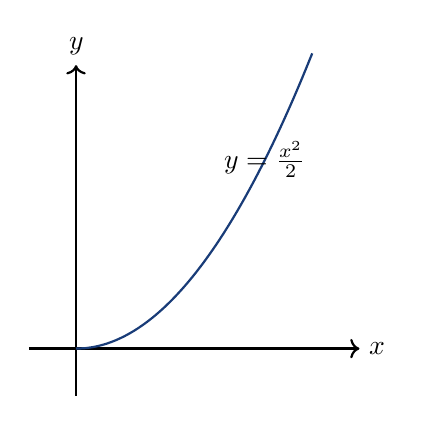
\begin{tikzpicture}[scale=1.2]
  \draw[thick,->] (-0.5,0) -- (3,0) node[right] {$x$};
  \draw[thick,->] (0,-0.5) -- (0,3) node[above] {$y$};
  \draw[domain=0:2.5,smooth,variable=\x,mainblue,thick]
    plot ({\x}, {\x*\x/2});
  \node at (2,2) {$y=\frac{x^2}{2}$};
\end{tikzpicture}
\end{frame}
\section{Circuit}
\begin{frame}{Circuit Example}
\centering
\begin{circuitikz}
\draw (0,0) node[ground]{} (0,0) node[above]{Earth Ground};
\draw (5,0) node[sground]{} (5,0) node[above]{Signal Ground};
\draw (10,0) node[cground]{} (10,0) node[above]{Chassis Ground};
\end{circuitikz}
\end{frame}
\section{Code}
\begin{frame}[fragile]{Code Example}
\centering
\begin{lstlisting}[language=C++]
#include<cstdio>
int main() {
  char a = 'a';
  printf("var a at %p is %c\n", (void*)&a, a);
  return 0;
}
\end{lstlisting}
\end{frame}
\section{Table}
\begin{frame}{Table Example}
\centering
\begin{longtable}{|c|c|}
\hline
Material medium & Refractive index\\\hline\endhead
Air & 1.0003\\\hline
Ice & 1.31\\\hline
Water & 1.33\\\hline
Alcohol & 1.36\\\hline
Kerosene & 1.44\\\hline
Fused quartz & 1.46\\\hline
Turpentine oil & 1.47\\\hline
Benzene & 1.50\\\hline
Crown glass & 1.52\\\hline
Diamond & 2.42\\\hline
\end{longtable}
\end{frame}
\section{Picture}
\begin{frame}{Picture}
\begin{center}

\includegraphics[height=0.5\textheight]{Tux.svg.png}
\end{center}
\end{frame}
\section{Conclusion}
\begin{frame}{Summary}
\begin{itemize}
  \item Clean structure
  \item Strong math support
  \item Highly customizable
\end{itemize}
\end{frame}
\begin{frame}
\centering
\Huge Questions?
\end{frame}
\end{document}